\documentclass[11pt,landscape,twocolumn,letterpaper]{article}

\usepackage[margin=1.27cm]{geometry}
\setlength{\textwidth}{10.0in}		% default=9in

\setlength{\columnsep}{0.5in}		% default=10pt
\setlength{\columnseprule}{0pt}		% default=0pt (no line)
%\setlength{\columnseprule}{0.2pt}		% default=0pt (no line)

\setlength{\textheight}{7in}		% default=5.15in
\setlength{\topmargin}{-.5in}		% default=0.20in

\setlength{\headsep}{0in}		% default=0.35in

\setlength{\parskip}{1.2ex}
\setlength{\parindent}{0mm}
\usepackage{graphicx}

%\usepackage{helvetica,color}
%\usepackage{newcent,color}
%\usepackage{bookman,color}
\usepackage{palatino}
\usepackage{color}
\usepackage{stmaryrd}
\pagestyle{empty}

\begin{document}
%\maketitle

\begin{center}
\textbf{Deuteronomy}
\end{center}
Deuteronomy consists of the parting counsels of Moses delivered to Israel in view of the impending entrance upon their covenanted possession. It contains a summary of the wilderness wanderings of Israel, which is important as unfolding the moral judgement of God upon those events; repeats the Decalogue to a generation which had grown up in the wilderness; gives needed instruction as the conduct of Israel in the land, and contains the Palestinian Covenant (Deuteronomy 30:1-9). The book breathes the sternness of the Law. Keywords, "Thou shalt"; key-verses, Deuteronomy 11:26-28 . It is important to note that, while the land of promise was unconditionally given Abraham and to his seed in the Abrahamic Covenant (Genesis 13:15 ; 15:7), it was under the conditional Palestinian Covenant (Deuteronomy 28:1-30:9) that Israel entered the land under Joshua. Utterly violating the conditions of that covenant, the nation was first disrupted (1 Kings 12) and then cast out of the land (2 Kings 17:1-18, 24:1-25:11). But the same covenant unconditionally promises a national restoration of Israel which is yet to be fulfilled (See Scofield). \textbf{Deuteronomy} has seven divisions: (I) Summary of the history of Israel in the wilderness, 1:1-3:29 (II) A restatement of the Law, with warnings and exhortations, 4:1-11:32, (III) Instructions, Warnings, and Predictions, 12:1-27:26, (IV) The great closing prophecies summarizing the history of Israel to the second coming of Christ, and containing the Palestinian Covenant, 28:1-30:20, (V) Last counsels to Priests, Levites, and to Joshua, 31, (VI) The Song of Moses and his parting blessings, 32-33, (VII) The Death of Moses, 34. 

\begin{tabular}{p{0.85in}p{1.25in}p{1.2in}p{1.2in}}
DATE & CHAPTERS & PSALM & PROVERB \\
\tiny 060 \normalsize Tue, $1^{st}$ & $\boxempty$ $\boxempty$ $\boxempty$ \hspace{.05in} \textcolor[rgb]{1.00,0.00,0.00}{Deut 22-24} & $\boxempty$ \hspace{.05in} \textcolor[rgb]{0.00,1.00,0.00}{Ps 60} &  $\boxempty$ \hspace{.05in} \textcolor[rgb]{0.00,0.00,1.00}{Prov 1}   \\

\tiny 061 \normalsize Wed, $2^{nd}$ & $\boxempty$ $\boxempty$ $\boxempty$ \hspace{.05in} \textcolor[rgb]{1.00,0.00,0.00}{Deut 25-27} & $\boxempty$ \hspace{.05in} \textcolor[rgb]{0.00,1.00,0.00}{Ps 61} &  $\boxempty$ \hspace{.05in} \textcolor[rgb]{0.00,0.00,1.00}{Prov 2}   \\

\tiny 062 \normalsize Thu, $3^{rd}$ & $\boxempty$ $\boxempty$ $\boxempty$ \hspace{.05in} \textcolor[rgb]{1.00,0.00,0.00}{Deut 28-30} & $\boxempty$ \hspace{.05in} \textcolor[rgb]{0.00,1.00,0.00}{Ps 62} &  $\boxempty$ \hspace{.05in} \textcolor[rgb]{0.00,0.00,1.00}{Prov 3}   \\

\tiny 063 \normalsize Fri, $4^{th}$ & $\boxempty$ $\boxempty$ $\boxempty$ \hspace{.05in} \textcolor[rgb]{1.00,0.00,0.00}{Deut 31-32} & $\boxempty$ \hspace{.05in} \textcolor[rgb]{0.00,1.00,0.00}{Ps 63} &  $\boxempty$ \hspace{.05in} \textcolor[rgb]{0.00,0.00,1.00}{Prov 4}   \\

\tiny 064 \normalsize Sat, $5^{th}$ & $\boxempty$ $\boxempty$ $\boxempty$ \hspace{.05in} \textcolor[rgb]{1.00,0.00,0.00}{Deut 33-34} & $\boxempty$ \hspace{.05in} \textcolor[rgb]{0.00,1.00,0.00}{Ps 64} &  $\boxempty$ \hspace{.05in} \textcolor[rgb]{0.00,0.00,1.00}{Prov 5}   \\

\end{tabular} 

\newpage
\begin{center}
\textbf{Joshua \& Judges}
\end{center}
\textbf{Joshua} records the consummation of the redemption of Israel of Israel out of Egypt; for redemption has two parts: "out," and "into" (Deuteronomy 6:23). The key-phrase is "Moses My servant is dead" (Joshua 1:2). Law, of which Moses is the representative, could never give a sinful people victory (Hebrews 7:19; Romans 6:14; 8:2-4).In a spiritual sense the book of Joshua is the Ephesians of the Old Testament. "The heavenly" of Ephesians is to the Christian what Canaan was to the Israelite and blessing through divine power (Joshua 21:43-55, Ephesians 1:3). \textbf{Judges} takes its name from the thirteen men raised up to deliver Israel in the declension and disunion which followed the death of Joshua. Through these men Jehovah continued His personal government of Israel. The key-verse to the condition of Israel is (Judges 17:6), "Every man did that which was right in his own eyes." The book records seven apostasies, seven servitudes to seven heathen nations, seven deliverances. The spiritual parallel is found in the history of the professing church since the Apostles (1 Corinthians 12:12-13).
\begin{tabular}{p{0.85in}p{1.25in}p{1.2in}p{1.2in}}
DATE & CHAPTERS & PSALM & PROVERB \\
\tiny 065 \normalsize Sun, $6^{th}$ & $\boxempty$ $\boxempty$ $\boxempty$ \hspace{.05in} \textcolor[rgb]{1.00,0.00,0.00}{Josh 1-3} & $\boxempty$ \hspace{.05in} \textcolor[rgb]{0.00,1.00,0.00}{Ps 65} & $\boxempty$ \hspace{.05in} \textcolor[rgb]{0.00,0.00,1.00}{Prov 6}  \\

\tiny 066 \normalsize Mon, $7^{th}$ & $\boxempty$ $\boxempty$ $\boxempty$ \hspace{.05in} \textcolor[rgb]{1.00,0.00,0.00}{Josh 4-6} & $\boxempty$ \hspace{.05in} \textcolor[rgb]{0.00,1.00,0.00}{Ps 66} & $\boxempty$ \hspace{.05in} \textcolor[rgb]{0.00,0.00,1.00}{Prov 7}  \\

\tiny 067 \normalsize Tue, $8^{th}$ & $\boxempty$ $\boxempty$ $\boxempty$ \hspace{.05in} \textcolor[rgb]{1.00,0.00,0.00}{Josh 7-9} & $\boxempty$ \hspace{.05in} \textcolor[rgb]{0.00,1.00,0.00}{Ps 67} & $\boxempty$ \hspace{.05in} \textcolor[rgb]{0.00,0.00,1.00}{Prov 8}  \\

\tiny 068 \normalsize Wed, $9^{th}$ & $\boxempty$ $\boxempty$ $\boxempty$ \hspace{.05in} \textcolor[rgb]{1.00,0.00,0.00}{Josh 10-12} & $\boxempty$ \hspace{.05in} \textcolor[rgb]{0.00,1.00,0.00}{Ps 68} & $\boxempty$ \hspace{.05in} \textcolor[rgb]{0.00,0.00,1.00}{Prov 9}  \\

\tiny 069 \normalsize Thu, $10^{th}$ & $\boxempty$ $\boxempty$ $\boxempty$ \hspace{.05in} \textcolor[rgb]{1.00,0.00,0.00}{Josh 13-15} & $\boxempty$ \hspace{.05in} \textcolor[rgb]{0.00,1.00,0.00}{Ps 69} & $\boxempty$ \hspace{.05in} \textcolor[rgb]{0.00,0.00,1.00}{Prov 10}  \\

\tiny 070 \normalsize Fri, $11^{th}$ & $\boxempty$ $\boxempty$ $\boxempty$ \hspace{.05in} \textcolor[rgb]{1.00,0.00,0.00}{Josh 16-18} & $\boxempty$ \hspace{.05in} \textcolor[rgb]{0.00,1.00,0.00}{Ps 70} & $\boxempty$ \hspace{.05in} \textcolor[rgb]{0.00,0.00,1.00}{Prov 11}  \\

\tiny 071 \normalsize Sat, $12^{th}$ & $\boxempty$ $\boxempty$ $\boxempty$ \hspace{.05in} \textcolor[rgb]{1.00,0.00,0.00}{Josh 19-21} & $\boxempty$ \hspace{.05in} \textcolor[rgb]{0.00,1.00,0.00}{Ps 71} & $\boxempty$ \hspace{.05in} \textcolor[rgb]{0.00,0.00,1.00}{Prov 12}  \\

\tiny 072 \normalsize Sun, $13^{th}$ & $\boxempty$ $\boxempty$ $\boxempty$ \hspace{.05in} \textcolor[rgb]{1.00,0.00,0.00}{Josh 22-24} & $\boxempty$ \hspace{.05in} \textcolor[rgb]{0.00,1.00,0.00}{Ps 72} & $\boxempty$ \hspace{.05in} \textcolor[rgb]{0.00,0.00,1.00}{Prov 13}  \\

\tiny 073\normalsize Mon, $14^{th}$ & $\boxempty$ $\boxempty$ $\boxempty$ \hspace{.05in} \textcolor[rgb]{1.00,0.00,0.00}{Jdgs 1-3} & $\boxempty$ \hspace{.05in} \textcolor[rgb]{0.00,1.00,0.00}{Ps 73} & $\boxempty$ \hspace{.05in} \textcolor[rgb]{0.00,0.00,1.00}{Prov 14}  \\

\tiny 074 \normalsize Tue, $15^{th}$ & $\boxempty$ $\boxempty$ $\boxempty$ \hspace{.05in} \textcolor[rgb]{1.00,0.00,0.00}{Jdgs 4-6} & $\boxempty$ \hspace{.05in} \textcolor[rgb]{0.00,1.00,0.00}{Ps 74} & $\boxempty$ \hspace{.05in} \textcolor[rgb]{0.00,0.00,1.00}{Prov 15}  \\

\tiny 075 \normalsize Wed, $16^{th}$ & $\boxempty$ $\boxempty$ $\boxempty$ \hspace{.05in} \textcolor[rgb]{1.00,0.00,0.00}{Jdgs 7-9} & $\boxempty$ \hspace{.05in} \textcolor[rgb]{0.00,1.00,0.00}{Ps 75} & $\boxempty$ \hspace{.05in} \textcolor[rgb]{0.00,0.00,1.00}{Prov 16}  \\

\tiny 076 \normalsize Thu, $17^{th}$ & $\boxempty$ $\boxempty$ $\boxempty$ \hspace{.05in} \textcolor[rgb]{1.00,0.00,0.00}{Jdgs 10-12} & $\boxempty$ \hspace{.05in} \textcolor[rgb]{0.00,1.00,0.00}{Ps 76} & $\boxempty$ \hspace{.05in} \textcolor[rgb]{0.00,0.00,1.00}{Prov 17}  \\

\tiny 077 \normalsize Fri, $18^{nd}$ & $\boxempty$ $\boxempty$ $\boxempty$ \hspace{.05in} \textcolor[rgb]{1.00,0.00,0.00}{Jdgs 13-15} & $\boxempty$ \hspace{.05in} \textcolor[rgb]{0.00,1.00,0.00}{Ps 77} & $\boxempty$ \hspace{.05in} \textcolor[rgb]{0.00,0.00,1.00}{Prov 18}  \\

\tiny 078 \normalsize Sat, $19^{th}$ & $\boxempty$ $\boxempty$ $\boxempty$ \hspace{.05in} \textcolor[rgb]{1.00,0.00,0.00}{Jdgs 16-18} & $\boxempty$ \hspace{.05in} \textcolor[rgb]{0.00,1.00,0.00}{Ps 78} & $\boxempty$ \hspace{.05in} \textcolor[rgb]{0.00,0.00,1.00}{Prov 19}  \\

\tiny 079 \normalsize Sun, $20^{th}$ & $\boxempty$ $\boxempty$ $\boxempty$ \hspace{.05in} \textcolor[rgb]{1.00,0.00,0.00}{Jdgs 19-21} & $\boxempty$ \hspace{.05in} \textcolor[rgb]{0.00,1.00,0.00}{Ps 79} & $\boxempty$ \hspace{.05in} \textcolor[rgb]{0.00,0.00,1.00}{Prov 20}  \\

\end{tabular}  
\newpage

\begin{center}
\textbf{Ruth}
\end{center}
This lovely story should be read in connection with the first half of Judges, as it presents a picture of life in Israel at that time. Typically, the book may be taken as a foreview of the church (Ruth), as the Gentile bride of Christ. Ruth also gives a normal Christian experience: (1) Ruth deciding, 1; (2) Ruth serving, 2; (3) Ruth resting, 3; (4) Ruth rewarded, 4. The events recorded in Ruth cover a period of 10 years (Ussher).
\begin{tabular}{p{0.85in}p{1.25in}p{1.2in}p{1.2in}}
DATE & CHAPTERS & PSALM & PROVERB \\
\tiny 080 \normalsize Mon, $21^{st}$ & $\boxempty$ $\boxempty$ $\boxempty$ \hspace{.05in} \textcolor[rgb]{1.00,0.00,0.00}{Ruth 1-2} & $\boxempty$ \hspace{.05in} \textcolor[rgb]{0.00,1.00,0.00}{Ps 80} & $\boxempty$ \hspace{.05in} \textcolor[rgb]{0.00,0.00,1.00}{Prov 21}  \\

\tiny 081 \normalsize Tue, $22^{nd}$ & $\boxempty$ $\boxempty$ $\boxempty$ \hspace{.05in} \textcolor[rgb]{1.00,0.00,0.00}{Ruth 3-4} & $\boxempty$ \hspace{.05in} \textcolor[rgb]{0.00,1.00,0.00}{Ps 81} & $\boxempty$ \hspace{.05in} \textcolor[rgb]{0.00,0.00,1.00}{Prov 22}  \\
\end{tabular} 

\begin{center}
\textbf{1 Samuel}
\end{center}
This book represents the personal history of Samuel. It records the moral failure of the priesthood under Eli, and of the Judges in Samuel's attempt to make the office hereditary (1 Samuel 8:1). Samuel begins the line of writing prophets. Henceforth the prophet, not the priest, is conspicuous in Israel. In this book the theocracy, as exercised through judges, ends (1 Samuel 8:7), and the line of kings begins with Saul. The book is in four parts: (1) The story of Samuel to the death of Eli, 1:1-4:22; (2) From the taking of the ark to the demand for a king, 5:1-8:22; (23) The reign of Saul to the call of David, 9:1-15:35; (4) From the call of David to the death of Saul, 16:1-31:13. The events recorded in First Samuel cover a period of 115 years (Ussher). 

\begin{tabular}{p{0.8in}p{1.3in}p{1.2in}p{1.2in}}
DATE & CHAPTERS & PSALM & PROVERB \\
\tiny 082 \normalsize Wed, $23^{rd}$ & $\boxempty$ $\boxempty$ $\boxempty$ \hspace{.05in} \textcolor[rgb]{1.00,0.00,0.00}{1Sam 1-3} & $\boxempty$ \hspace{.05in} \textcolor[rgb]{0.00,1.00,0.00}{Ps 82} & $\boxempty$ \hspace{.05in} \textcolor[rgb]{0.00,0.00,1.00}{Prov 23}  \\

\tiny 083 \normalsize Thu, $24^{rd}$ & $\boxempty$ $\boxempty$ $\boxempty$ \hspace{.05in} \textcolor[rgb]{1.00,0.00,0.00}{1Sam 4-6} & $\boxempty$ \hspace{.05in} \textcolor[rgb]{0.00,1.00,0.00}{Ps 83} & $\boxempty$ \hspace{.05in} \textcolor[rgb]{0.00,0.00,1.00}{Prov 24}  \\

\tiny 084 \normalsize Fri, $25^{th}$ & $\boxempty$ $\boxempty$ $\boxempty$ \hspace{.05in} \textcolor[rgb]{1.00,0.00,0.00}{1Sam 7-9} & $\boxempty$ \hspace{.05in} \textcolor[rgb]{0.00,1.00,0.00}{Ps 84} & $\boxempty$ \hspace{.05in} \textcolor[rgb]{0.00,0.00,1.00}{Prov 25}  \\

\tiny 085 \normalsize Sat, $26^{th}$ &  $\boxempty$ $\boxempty$ $\boxempty$ \hspace{.05in} \textcolor[rgb]{1.00,0.00,0.00}{1Sam 10-12} &  $\boxempty$ \hspace{.05in} \textcolor[rgb]{0.00,1.00,0.00}{Ps 85} &  $\boxempty$ \hspace{.05in} \textcolor[rgb]{0.00,0.00,1.00}{Prov 26}  \\

\tiny 086 \normalsize Sun, $27^{th}$ &  $\boxempty$ $\boxempty$ $\boxempty$ \hspace{.05in} \textcolor[rgb]{1.00,0.00,0.00}{1Sam 13-15} &  $\boxempty$ \hspace{.05in} \textcolor[rgb]{0.00,1.00,0.00}{Ps 86} &  $\boxempty$ \hspace{.05in} \textcolor[rgb]{0.00,0.00,1.00}{Prov 27}  \\

\tiny 087 \normalsize Mon, $28^{th}$ &  $\boxempty$ $\boxempty$ $\boxempty$ \hspace{.05in} \textcolor[rgb]{1.00,0.00,0.00}{1Sam 16-18} &  $\boxempty$ \hspace{.05in} \textcolor[rgb]{0.00,1.00,0.00}{Ps 87} &  $\boxempty$ \hspace{.05in} \textcolor[rgb]{0.00,0.00,1.00}{Prov 28}  \\

\tiny 088 \normalsize Tue, $29^{th}$ &   $\boxempty$ $\boxempty$ $\boxempty$ \hspace{.05in} \textcolor[rgb]{1.00,0.00,0.00}{1Sam 19-21} & $\boxempty$ \hspace{.05in} \textcolor[rgb]{0.00,1.00,0.00}{Ps 88} & $\boxempty$ \hspace{.05in} \textcolor[rgb]{0.00,0.00,1.00}{Prov 29}  \\

\tiny 089 \normalsize Wed, $30^{th}$ &  $\boxempty$ $\boxempty$ $\boxempty$ \hspace{.05in} \textcolor[rgb]{1.00,0.00,0.00}{1Sam 22-24} &  $\boxempty$ \hspace{.05in} \textcolor[rgb]{0.00,1.00,0.00}{Ps 89} &  $\boxempty$ \hspace{.05in} \textcolor[rgb]{0.00,0.00,1.00}{Prov 30}  \\

\tiny 090 \normalsize Thu, $31^{st}$ &   $\boxempty$ $\boxempty$ $\boxempty$ \hspace{.05in} \textcolor[rgb]{1.00,0.00,0.00}{1Sam 25-27} & $\boxempty$ \hspace{.05in} \textcolor[rgb]{0.00,1.00,0.00}{Ps 90} & $\boxempty$ \hspace{.05in} \textcolor[rgb]{0.00,0.00,1.00}{Prov 31}  \\
\end{tabular} 
\newpage

\LARGE
\begin{center}
\textcolor[rgb]{0.98,0.00,0.00}{Daily Bible Reading -- Plan B}\\
\textcolor[rgb]{0.00,0.00,1.00}{March 2022}\\
\end{center}

\begin{figure}[htp]
    \centering
  % Requires \usepackage{graphicx}
  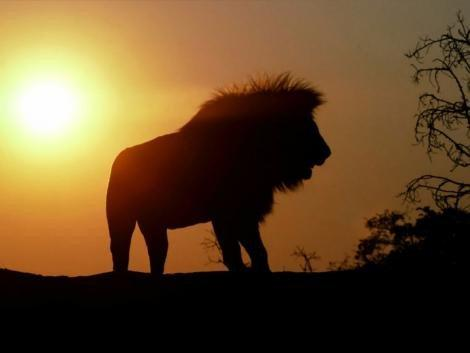
\includegraphics[width=4.5in]{March}\\
%  \caption{}\label{}
\end{figure}

\begin{center}
\textcolor[rgb]{0.00,0.00,1.00}{\\Ask Yourself ...}
\textcolor[rgb]{1.00,0.00,0.00}{\\Who is Speaking?\\Who is being spoken to?\\What is being said?\\Are there
any commandments to obey?\\Are there any promises to claim?}
\end{center}


\end{document}
